\chapter{Planaridad local}

\comm{davenma y venema}

\begin{df}
Dados dos cerrados $A$, $B$ de un espacio $X$, consideramos en $A\times[0,1]$ la relación de equivalencia cuyas clases no triviales están dadas por $$(x,t)\sim (x,t')\iff x\in A\cap B$$
Llamamos \textbf{collar de A pinchado en B} a un encaje $h\colon A\times[0,1]/_{\sim}\to X$ tal que \begin{itemize}
\item $h(x,0)=x$ para todo $x\in A$
\item $h(A\times [0,1]/_\sim)$ es un entorno de $A - B$
\end{itemize}
\end{df} \duda{buscar una mejor traducción, en realidad es pinched collar}

\begin{lema}
	Sean $A$, $B$ cerrados de $X$ tal que $A$ tiene entornos de collar locales en $X$ para todo punto de $A-B$. Entonces, existe un collar de $A$ pinchado en $B$.
\end{lema}

\begin{lema}
	Sea $h\colon\Delta^n\to \s^n$, con $n\geq 4$, un encaje de un $n$-símplice en $\s^n$ tal que es lineal a trozos en todo $\Delta^n$ salvo un vértice. Entonces, $\s^n - \mathring{(\Delta^n)}$ es una $n$-bola.
\end{lema}

\begin{proof}
Sea $h\colon\Delta^n\to\s^n$ un encaje que es lineal a trozos en $\Delta^n - \{v\}$ para $v$ un vértice de $\Delta^n$. 

Tomamos $A$ un $n$-símplice tal que $\Delta^n\subset A$ y $\partial A\cap\Delta^n=\{v\}$ como en la imagen \ref{simp1}.

Sea $B$ un $n$-símplice contenido en el interior de $\Delta^n$. Dado un vértice $w\in B$, consideramos $\alpha$ el segmento lineal que va de $v$ a $w$. Como los símplices son convexos, a menos de algunos ajustes podemos asegurarnos que $\alpha\cap B=\{w\}$, como en la imagen \ref{simp2}.

Como el encaje $h$ es lineal a trozos en todo $\Delta^n$ salvo $\{v\}$, sabemos que $h|_{\Delta^n - \{v\}}$ se extiende a un encaje lineal a trozos $\hat{h}$ de $\left(\Delta^n - \{v\}\right)\times [0,1]$, es decir, se extiende a un entorno collar de $\Delta^n - \{v\}$. Por el lema anterior entonces podemos decir que $\Delta^n$ tiene un entorno de collar pinchado en $\{v\}$. Convenientemente este entorno es como en la imagen \ref{simp1}, lo que nos dice que podemos ver $\hat{h}$ como un encaje topológico (no PL) de $A$ en $\s^n$. 

Por el lema anterior, el encaje $h$ 
\end{proof}

\begin{figure}
    	\centering
    	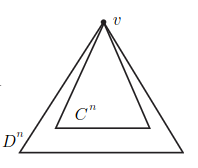
\includegraphics[width=0.35\linewidth]{img mono/casi plano/1.png}
    	\caption{Dibujito}
        \label{simp1}
\end{figure}

\begin{figure}
    	\centering
    	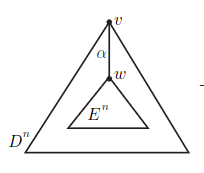
\includegraphics[width=0.35\linewidth]{img mono/casi plano/2.png}
    	\caption{Dibujito}
        \label{simp2}
\end{figure}



\comm{kirby}

Sea $C$ un subconjunto no vacío de un Cantor ternario estándar en $[-1,1]$. Supongamos que $\{-1,\,1\}\in C$. Tomamos $D:=\{d_1,d_2\dots\}$ un subconjunto numerable y denso en $[-1,1]\cap C^c$ (por ejemplo, tomar los puntos medios de los intervalos que se van eliminando para definir $C$).

Consideramos la siguiente curva $J$ en $\s^{n-1}$:
$$J:=\left\{(x_1,\dots, x_n)\in\s^n\subset\R^n\colon x_{n-1}^2+ x_{n}^2=1,\, x_{n-1}\geq 0, x_1=x_2=\dots = x_{n-2}=0\right\}$$

\begin{figure}
    	\centering
    	\includegraphics[width=0.4\linewidth]{img mono/kirby/j.png}
    	\caption{La curva $J$ en $\s^2$}
        \label{jota}
\end{figure}

Identificamos $[-1,1]$ con la 